\documentclass[11pt]{article}
\usepackage[letterpaper,margin=0.95in]{geometry}
\usepackage{amsmath,amssymb,booktabs,graphicx}
\usepackage[font=small,labelfont=bf]{caption}
\usepackage[hidelinks]{hyperref}
\hypersetup{pdftitle={Forecasting label changes under Gaussian prototype flows},pdfsubject={Finite-time label crossing and selective integration}}
\setlength{\emergencystretch}{2em}
\setcounter{topnumber}{3}
\renewcommand{\topfraction}{0.90}
\renewcommand{\textfraction}{0.08}
\renewcommand{\floatpagefraction}{0.78}
\newcommand{\R}{\mathbb{R}}
\newcommand{\Cov}{\operatorname{Cov}}
\newcommand{\tr}{\operatorname{tr}}
\newcommand{\AP}{\operatorname{AP}}
\newcommand{\dd}{\mathrm{d}}
\newcommand{\norm}[1]{\lVert #1\rVert}
\newcommand{\argmax}{\operatorname*{arg\,max}}
\title{Forecasting label changes under Gaussian prototype flows}
\author{}
\date{}
\begin{document}
\maketitle
\newcommand{\SynAP}{0.9966}
\newcommand{\PubAP}{0.9867}
\newcommand{\SynStaticAP}{0.4846}
\newcommand{\PubStaticAP}{0.5251}
\newcommand{\SynEtdAP}{0.9954}
\newcommand{\PubEtdAP}{0.9904}
\newcommand{\SynCover}{32.08\%}
\newcommand{\PubCover}{41.62\%}


\begin{abstract}
Gaussian prototype scores can define both a static classifier and a vector field that transports an input before classification. We study which labels change under this transport when prototypes are fitted on restricted class cores. At a regular leading tie, a closed-form normal derivative gives the local crossing direction. Posterior covariance bounds give sufficient tests in exact arithmetic for class preservation over a time interval and for the terminal label. Integrating the known linear part of the field yields a separate endpoint enclosure. A short-time risk calculation distinguishes label changes from their classification cost. We evaluate four new synthetic geometries and two public datasets with a locked protocol. At the primary setting, the projected margin ranked endpoint changes with mean average precision \SynAP{} on synthetic cases and \PubAP{} on public cases, versus \SynStaticAP{} and \PubStaticAP{} for the initial margin and \SynEtdAP{} and \PubEtdAP{} for one exponential Euler step. The combined endpoint tests covered \SynCover{} and \PubCover{} of queries. The strict selective solver reduced field calls and increased measured latency. A fixed exponential Euler triage gate ran faster, with zero synthetic and one public label disagreement at the primary horizon. Its fidelity decreased at the longest horizon.
\end{abstract}

\section{Introduction}
Classifiers assign labels outside the parts of feature space represented by their training cores. Gaussian prototype scores can be read immediately at an external point or after following a density-ascent trajectory. These decisions share learned geometry and can disagree. A motivating pilot found this disagreement concentrated in the withheld wedges of a ring benchmark. This study treats the pilot as development evidence and evaluates new generators, public sources, and random seeds.

We ask three questions. Can the fitted scores and field predict the direction of a class-boundary crossing? What finite-time guarantees are available without integrating a query? What connects a crossing to an improvement or deterioration in class prediction? We derive a model-specific diagnostic and test it against matched static scores, numerical integrators, and controls of known class density. Predictions of crossing concern the classifier's own decision regions. Measuring classification harm additionally requires true external labels.

\paragraph{Related work.}
Gaussian mean shift follows ascent toward modes of a kernel density, and modal clustering studies the associated basins \cite{comaniciu,carreira,chacon}. Class decisions compare separate class masses. The total mixture can grow along a trajectory while the ranking of those masses changes. SA-nODE and SODEF use dynamical systems for classification and robustness, with different training goals and terminal rules \cite{marino,kang}. Joint Energy Models use a shared set of logits for the energy and prediction and evaluate stochastic input refinement \cite{jem}. We study a deterministic finite-time transport of fixed scores fitted on training cores. Finite-time ODEs with linear output have established topological limits on nested classes, and augmented and second-order dynamics can overcome the specific obstruction \cite{dupont,norcliffe}. Our output is a fixed nonlinear score and our claims concern crossings and finite-time enclosures. Exponential Euler and state-to-margin bounds are established numerical and verification tools \cite{cox,hochbruck,tsuzuku}. Neural ODE verification also checks classifier outputs using general reachability tools \cite{nnvode}. The proposed enclosure uses explicit covariance and diameter bounds specific to a Gaussian prototype field. Quadratic expansions of excess Bayes risk under boundary perturbation have established antecedents \cite{hall,samworth,setoudeh}. We specialize the expansion to flow transport and compare it with a first-order crossing law.

\section{Field, ties and transition rates}
Let $a_i\in\R^d$ be a prototype with class $c_i$ and mass $w_i>0$, and let $\beta>0$ be the common Gaussian variance. Set
\[
 S_c(x)=\sum_{i:c_i=c}w_i\exp\!\left(-\frac{\norm{x-a_i}^2}{2\beta}\right),\qquad
 g_c(x)=\beta\log S_c(x),\qquad C(x)=\argmax_c g_c(x).
\]
The marginal log-density gives the field
\[
 F(x)=\nabla\big[\beta\log\sum_c S_c(x)\big]=\mu(x)-x,\qquad
 \mu=\sum_c \pi_c\mu_c,\qquad \pi_c=\frac{S_c}{\sum_j S_j},
\]
where $\mu_c$ is the within-class posterior mean of the prototypes. We write $\Phi_t$ for the autonomous flow. Static and transported labels are $C(x)$ and $C(\Phi_t x)$, with a deterministic tie rule. Adding a common function to all $g_c$ preserves the static comparisons and changes their associated marginal field by the gradient of that function. The field in this study is fixed by the full Gaussian scores, including the common quadratic term.

For $m_{ba}=g_b-g_a$ and $v_c=\mu_c-x$,
\begin{equation}
 \frac{\dd}{\dd t}m_{ba}(\Phi_t x)\bigg|_{t=0}=(v_b-v_a)^\top F(x).
 \label{eq:direction}
\end{equation}
On a regular top tie $g_a=g_b>\max_{j\notin\{a,b\}}g_j$, the sign of \eqref{eq:direction}, when nonzero, gives the crossing direction locally. In the binary case it is the sign of
\[
 \tfrac12(\norm{v_b}^2-\norm{v_a}^2).
\]
For multiple classes there is an additional term $\sum_{j\notin\{a,b\}}\pi_j(v_b-v_a)^\top v_j$, and the first term has coefficient $\pi_a=\pi_b$. A lower-scoring third class can reverse the crossing direction by changing the common vector field. As a concrete example at $x=0$, take posterior masses $(0.34,0.34,0.32)$ and one-dimensional conditional velocities $(1,0.4,-2)$, attainable with single sources and positive weights. The class-1 minus class-2 margin initially decreases because $F=-0.164$. It increases in the binary model obtained by keeping the two tied sources alone. Isolated tangencies, singular ties, and simultaneous leading ties require separate treatment.

Let $p_c$ denote the weighted joint density for class $c$, with $\rho=\sum_c p_c$. Equal class weighting uses $p_c=f_c/C$, where $f_c$ is the conditional feature density. For regular strict top faces $\Sigma_{ab}$ with unit normal $n_{ab}=\nabla m_{ba}/\norm{\nabla m_{ba}}$ toward $b$, the outgoing mass from $a$ to $b$ at short time is
\[
 t\int_{\Sigma_{ab}}\rho(F\cdot n_{ab})_+\,\dd S+o(t).
\]
With suitable local smoothness and integrability, the signed derivative of classification error is $\sum_{a<b}\int_{\Sigma_{ab}}(p_a-p_b)(F\cdot n_{ab})\,\dd S$. These formulas follow from the normal widths of the sets swept by the boundary and require the external feature or class density on that boundary. The fitted scores alone determine the orientation term in \eqref{eq:direction}.

\section{Finite-time bounds}
\label{sec:bounds}
A short-horizon score uses the instantaneous derivative $r_c=v_c^\top F$ and exponential time $u_t=1-e^{-t}$. We rank likely endpoint changes by
\[
 H_t(x)=\max_{b\ne C(x)}\{g_b+u_t r_b-g_{C(x)}-u_t r_{C(x)}\}.
\]
Ordinary time $t$ gives a first-order comparison. Reading the exact score at $q_t=x+u_t F(x)$ gives the numerical one-step exponential Euler comparison. All are computed without outcomes or trajectories.

\paragraph{A query-local tube.}
Let $D$ be the prototype diameter, $D_c$ a within-class diameter, and $D_{ab}$ the maximum distance between prototypes of classes $a,b$. The posterior covariance identity is
\[
 D\mu(x)=\Cov_{\pi(\cdot\mid x)}(a)/\beta,\qquad DF(x)=D\mu(x)-I.
\]
For any unit projection, variance is at most $D^2/4$ by the bounded range. The field is globally Lipschitz and all finite-time maps exist. The logits are affine up to a common term, and the range of their shifts on a ball of radius $R$ around a query is at most $DR/\beta$. Every posterior weight can therefore increase by at most $\exp(DR/\beta)$. Computing weighted variance about the original mean upper-bounds the shifted covariance by the corresponding original variance times this multiplier. In particular,
\[
 \norm{D\mu(z)}\le \kappa(R)=\frac1\beta\min\!\left(
 \frac{D^2}{4},\, e^{DR/\beta}\tr\Cov_{\pi(\cdot\mid x)}(a)\right).
\]
The analogous classwise bound uses $D_c$ and the conditional covariance. For $\lambda=\kappa-1$, $v_0=\norm{F(x)}$ and $I_\lambda(t)=\int_0^t e^{\lambda s}\,\dd s$, symmetry of $DF$ gives $\norm{F(\Phi_t x)}\le v_0e^{\lambda t}$ while inside a valid tube. We initialize it with the global rate and intersect with the independent radius $u_t\max_i\norm{a_i-x}$ from variation of constants and convexity of the prototype hull. Each use of a valid tube to compute a local rate gives another valid radius $v_0 I_\lambda(t)$. Intersecting these radii twice maintains enclosure throughout $[0,t]$.

\paragraph{Margin bounds.}
Put $G=\min(D_{ab},\norm{\nabla m_{ba}(x)}+H R)$ and let $H$ be the maximum of the class covariance bounds divided by $\beta$. The Hessian is the difference of two positive semidefinite matrices, so its spectral norm is bounded by the larger norm. We have $\norm{\nabla m_{ba}}\le G$ and $\norm{\nabla^2m_{ba}}\le H$ in the tube. Dots below denote derivatives along the flow. Since
\[
 \ddot m+\dot m=F^\top \nabla^2m\,F+\nabla m^\top D\mu\,F,
\]
we can integrate the linear part exactly. With $J_\lambda(t)=\int_0^t(1-e^{-(t-s)})e^{\lambda s}\,\dd s$,
\begin{equation}
 |m(\Phi_t x)-m(x)-u_t\dot m(x)|
 \le H v_0^2 J_{2\lambda}(t) + G\kappa v_0 J_\lambda(t).
 \label{eq:drag}
\end{equation}
For comparison, ordinary Taylor uses center $m(x)+t\dot m(x)$, $\max(1,\lambda)$ in place of $\kappa$, and the kernel $t-s$ in both integrals. For fixed tube constants the right side in \eqref{eq:drag} is convex in $u_t$. Its derivative with respect to $u_t$ is $\int_0^t e^s W(s)\,\dd s$ for the nonnegative residual envelope $W$. The Taylor error is convex in $t$. If all comparisons for the initial winner have strict positive lower bounds at the horizon, with a strict initial decision, the corresponding lower bounds remain positive throughout. Bounds from either construction can be used for each comparison. A rival certified to beat the initial winner at the horizon implies a departure by that time.

\paragraph{Endpoint state bound and decision.}
Duhamel's formula and the speed enclosure give
\[
 \norm{\Phi_t x-q_t}\le\kappa v_0 J_\lambda(t).
\]
Indeed, $z_t-q_t=\int_0^t e^{-(t-s)}[\mu(z_s)-\mu(x)]\,\dd s$ and the integrand is bounded by $\kappa v_0 I_\lambda(s)$. Consequently a margin computed at $q_t$ has endpoint error at most $D_{ab}\kappa v_0 J_\lambda(t)$. This condition can certify the terminal winner even on a trajectory that leaves its initial class and returns. We keep endpoint-only bounds out of the whole-interval preservation test. The diagnostic may maximize all three valid pairwise lower bounds for an endpoint. The faster selective solver uses only the state bound and integrates the remaining queries. Exact arithmetic is assumed in all proofs. The implementation centers coordinates, uses stable mixture weights and positive comparison slack, and is tested against a high-accuracy numerical reference.

\section{When a crossing increases risk}
\label{sec:bayes}
Assume the static ordering is the Bayes ordering of the $p_c$, the relevant top faces are regular, and the active junctions admit transverse local coordinates. Assume also that tails outside compact sets contribute a uniformly negligible remainder at the scale stated below. On a strict regular face, put $\gamma_{ab}=\norm{\nabla(p_b-p_a)}$. The constant term of $p_b-p_a$ vanishes at the tie. On the outgoing side its magnitude at normal distance $s$ is $\gamma_{ab}s+o(s)$. The exact excess-risk identity integrates the Bayes joint density minus the assigned joint density. Integrating this linear loss across the swept strip of width $t|F\cdot n|+O(t^2)$ gives
\begin{equation}
 R(C\circ\Phi_t)-R(C)=
 \frac{t^2}{2}\sum_{a<b}\int_{\Sigma_{ab}}\gamma_{ab}(F\cdot n_{ab})^2\,\dd S +o(t^2).
 \label{eq:regret}
\end{equation}
Transverse top junctions occupy an $O(t^2)$ volume with an $O(t)$ density gap, which gives $O(t^3)$ risk locally. Thus labels can change at a first-order rate while the excess Bayes error grows at a second-order rate. If $p_c$ is proportional to $S_c$ by the same positive factor for all classes, then $\gamma_{ab}=p_* \norm{\nabla m_{ba}}/\beta$ at the face of joint density $p_*$. Equation (2.7) in \cite{setoudeh} gives the same specialization by pulling back joint densities along the flow. The Jacobian term cancels for a density difference at a tie. The fitted evaluation makes no Bayes assumption about the partially observed cores.

\section{Locked experimental protocol}
Four synthetic families offer affine shells, wavy shells, open chains with nuisance coordinates, and separated lobes as a control. Each seed-family draw supplies three gaps of equal training size, keeping the same external test features and labels. The gap moves the observed bands and thereby changes the fitted scaler and prototypes. The primary synthetic design uses 144 family--gap--seed units and 17,280 distinct external rows. The transfer evaluation uses 24 family--seed units from UCI PenDigits and Seeds \cite{pendigits,seeds}. PenDigits retains the original source split by writer and samples 1,430 external rows across disjoint folds. Individual writer identities within the source folds are unavailable. Seeds uses 89 distinct external rows in 459 evaluations, sampled from a fixed holdout as the cores change. External rows are selected by the benchmark curator using true classes and training-side anchor radii and sampled for class balance. Only training features and labels enter model fitting. Group-level inference for independent new writers, harvests or producers is outside these cohorts.

For every fit, a scaler and three $k$-means prototypes per class use only the allowed core examples. Classes and prototypes within each class receive equal masses. Standard deviation is the prototype diameter times $0.30$ or $0.45$. The primary setting is $0.30$ at horizon $0.5$. Horizons $0.15$ and $1.25$ and the other bandwidth ratio are fixed sensitivity settings. Twelve final seed values are disjoint from the two development values. DOP853 at relative tolerance $2\cdot10^{-10}$ and absolute tolerance $3\cdot10^{-12}$ is the numerical reference. Regular tie probes from pairwise score roots are filtered by a positive gap to other classes and a minimum absolute derivative before forward simulation. Whole-path preservation is checked at fixed trajectory checkpoints. The proof supplies continuous-time coverage on certified rows in exact arithmetic. Sampled checkpoints cannot rule out arbitrary recrossings.

The three deployment comparisons use fixed-step RK4 with step at most $0.1$, the state-bound guard with the same RK4 fallback, and an empirical triage gate. Triage integrates if the one-step exponential Euler projection loses the initial class lead or retains a lead of at most $0.1$ in log-score units. Direct one-step inference is reported separately. Measures include field evaluation count, median single-thread batch latency, and label disagreement against DOP853. The field count records a guard's initial field computation. It excludes score, bound and allocation overhead. Relative timings include that overhead. The locking rule for a strict speed claim includes 50\% endpoint coverage, 40\% fewer field evaluations, a ten percent latency saving, and numerical agreement. The ranking gate is a mean AP increment of at least $0.2$ over the initial margin. AP is computed on units with both endpoint changes and nonchanges and averaged across those units. Seed-block intervals keep dependencies across gaps and settings. Public intervals are conditional on the fixed data sources.

The known-law calibration uses four one-dimensional Gaussian mixtures with symmetric binary, asymmetric-prior binary, multimodal binary and multiclass faces. It enumerates all relevant ties using analytic single-source roots or sign-variation bounds saturated by root brackets. Ordered preimages of the active ties identify the swept intervals. Gaussian CDFs yield total risk. Local quadrature of density differences independently checks the small excess. These fixtures evaluate the coefficients of the two asymptotic laws with known densities.

\section{Results}
\label{sec:results}
\subsection{Crossing forecasts transfer across the tested geometries}
At the primary setting the exact tie direction agreed with the small forward probe on all 7,144 eligible synthetic and 1,007 eligible public top ties. The counts are over accepted pairwise root probes, which may visit the same boundary region. No quantitative claim is made about ties excluded by the derivative or top-gap conditions.

The main query-level result was the improvement in ranking endpoint changes over initial ambiguity (Figure~\ref{fig:forecast} and Table~\ref{tab:rank}). On synthetic units with both outcomes, the projected margin's AP was $0.9966$, versus $0.4846$ for the negative initial margin. The equal-seed difference was $0.5120$ with interval $[0.4911,0.5332]$. The public unit-macro AP values were $0.9867$ and $0.5251$, with an equal-seed difference of $0.4576$ and interval $[0.3798,0.5360]$. These mean APs average the 108 synthetic and 20 public units containing both outcomes, at mean change prevalences 16.42\% and 8.03\%. The four omitted public units and the separated-lobe control had no eligible mixed outcome. Ordinary linear projection reached $0.9849$ and $0.9891$, and exponential Euler reached $0.9954$ and $0.9904$. The comparison supports the use of a one-step directional forecast over static uncertainty. It gives little evidence of a practically meaningful ranking advantage over exponential Euler.

\begin{table}[htbp]
\centering
\small
\caption{Primary regime. AP is averaged over units with both endpoint changes and nonchanges. The final column gives transported minus static balanced accuracy. Labels in the first three AP columns describe forecasts of changes relative to the solver, not class labels.}
\label{tab:rank}
\begin{tabular}{lrrrrr}
\toprule
Family & Mixed units & Initial AP & Projected AP & ETD1 AP & BA shift (pp)\\
\midrule
Affine shells & 36 & .4581 & .9990 & .9994 & $+7.43$\\
Wavy shells & 36 & .5460 & .9995 & .9986 & $-4.77$\\
Open chains & 36 & .4498 & .9915 & .9881 & $-1.06$\\
Separated lobes & 0 & -- & -- & -- & $0.00$\\
PenDigits & 12 & .4839 & .9779 & .9841 & $-2.43$\\
Seeds & 8 & .5869 & 1.0000 & 1.0000 & $-1.79$\\
\bottomrule
\end{tabular}
\end{table}

\begin{figure}[htbp]
\centering
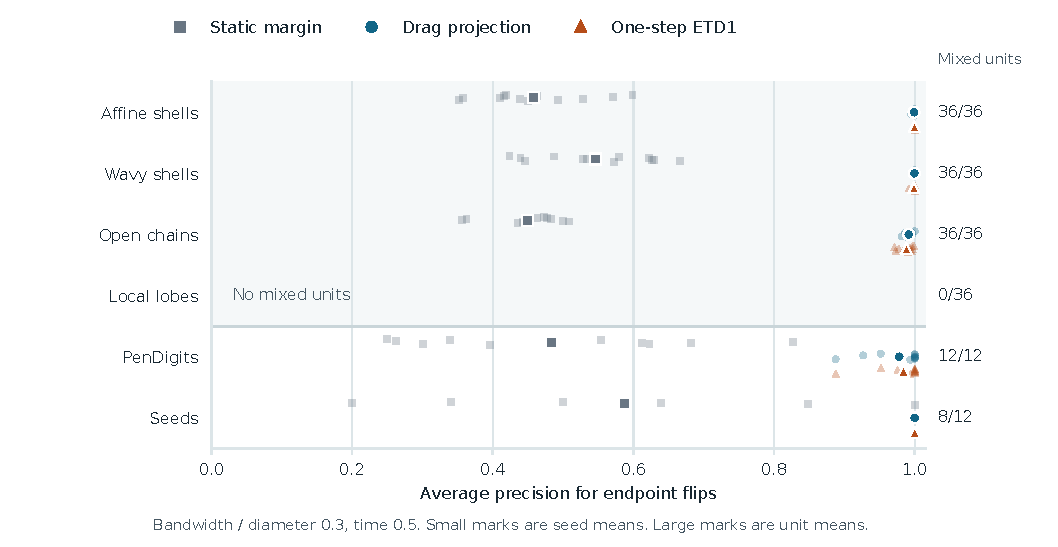
\includegraphics[width=\linewidth]{figures/forecast.pdf}
\caption{Prospective endpoint-change ranking at the primary bandwidth and horizon. Unit-level AP is undefined for units without both outcomes. ETD1 reads the class scores after one exponential Euler step.}
\label{fig:forecast}
\end{figure}

\subsection{Enclosures cover many stable queries and rarely prove a primary-horizon departure}
We observed no certificate contradictions against the numerical reference at any locked setting. At the primary horizon the combination certified the terminal label for 32.08\% of synthetic and 41.62\% of public query units on average. Whole-interval coverage exceeded that of the displacement-only ball by 5.83 percentage points (seed interval $[4.98,6.74]$) and 34.19 points ($[30.91,37.38]$). The combined terminal-label tests exceeded ordinary Taylor coverage by 0.04 and 0.23 points at this setting. Most certificates established preservation. Of 6,383 synthetic and 140 public endpoint changes, just 19 and zero were certified departures at this horizon. At horizon $0.15$ and bandwidth ratio $0.30$, the counts were 700 of 2,090 and 6 of 34. Figure~\ref{fig:certification} shows the dependence on scale and horizon. One primary case in each stage sampled a changed label that later returned. Endpoints alone would miss those cases.

\begin{figure}[htbp]
\centering
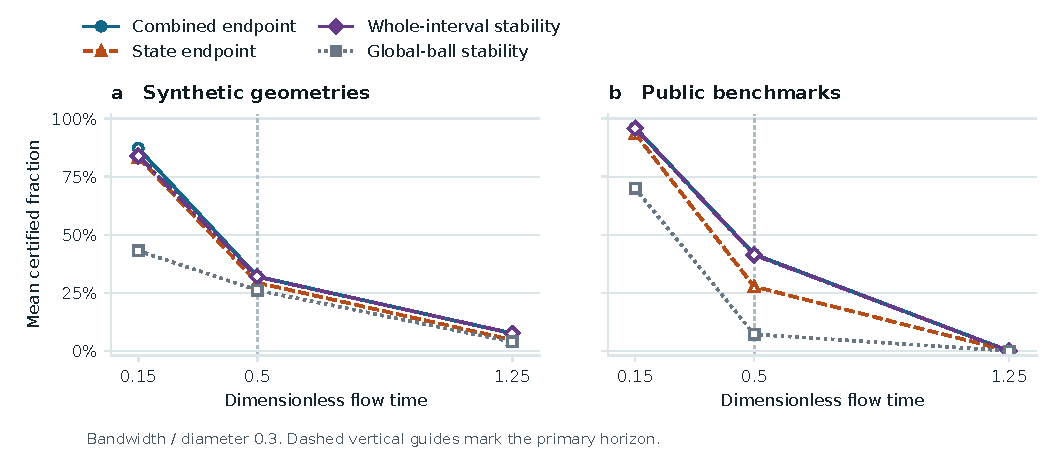
\includegraphics[width=\linewidth]{figures/certification.pdf}
\caption{Terminal-label and whole-interval coverage across the preregistered horizons. A terminal label can be certified after a return to the initial class. A stability certificate excludes any departure during the interval.}
\label{fig:certification}
\end{figure}

\subsection{A field-call saving can lose time}
The selective state-bound guard reduced field calls by 24.43\% on synthetic queries and 22.72\% on public queries, with no observed primary label mismatches to DOP853 (Table~\ref{tab:cost}). Its median batch latency ratios to unguarded RK4 were $1.32$ and $1.42$. The coverage and efficiency gates for a strict deployment advantage failed in both stages. Coverage is concentrated in easy regions. At the primary setting the combined diagnostic covered every separated-lobe query, whereas coverage on the open chains was 0.42\%. The guarded solver was faster than full RK4 in the lobe control and slower on the other primary families at their median settings.

The empirical triage policy gave a different fidelity--cost trade-off. The median latency ratios were $0.52$ and $0.69$, with zero synthetic disagreements in 51,840 primary query evaluations and one public disagreement in 1,889. Direct ETD1 readout was faster and disagreed on 637 and 25 of those evaluations. At $t=1.25$ and bandwidth ratio $0.30$, triage disagreed on 561 synthetic and 41 public evaluations. The shorter-horizon finding is therefore conditional on the tested setting. Triage is a fixed numerical heuristic without the guard's continuous-time guarantee. Query totals count repeated settings and held-out points used across gaps. They do not provide an independent-sample bound on triage error in new deployment domains.

\begin{table}[htbp]
\centering
\small
\caption{Primary numerical fidelity and cost. Latency ratios are medians of paired task-seed batch ratios versus fixed-step RK4. Disagreements compare each output with DOP853.}
\label{tab:cost}
\begin{tabular}{lrrrr}
\toprule
 & \multicolumn{2}{c}{Synthetic ($n=51{,}840$)} & \multicolumn{2}{c}{Public ($n=1{,}889$)}\\
Rule & Time ratio & Disagreements & Time ratio & Disagreements\\
\midrule
RK4 & 1.00 & 0 & 1.00 & 0\\
State-bound guard + RK4 & 1.32 & 0 & 1.42 & 0\\
One-step exponential Euler & 0.12 & 637 & 0.14 & 25\\
Projection triage + RK4 & 0.52 & 0 & 0.69 & 1\\
\bottomrule
\end{tabular}
\end{table}

\subsection{External class risk depends on the geometry and the underlying label law}
Transport improved balanced accuracy by 7.43 points on affine shells and reduced it by 4.77 on wavy shells. The paired largest-minus-smallest gap contrast in net harm averaged $+3.82$ points over the two shell families, with seed interval $[-4.68,+12.26]$. The shell-family point estimates were $+10.16$ on affine and $-2.52$ on wavy shells. At the primary setting the mean public decrease was $2.11$ points, with conditional seed interval $[1.11,3.28]$. These results did not establish a transferable law that widening the gap makes transport more harmful. They separate accurate identification of changed decisions from the weaker ability to predict the sign of the true-label effect.

In the known-law calibration, the symmetric binary tie was invariant and both coefficients were zero. The three nonzero cases checked both predicted coefficients to within 0.27\% relative error at the shortest measured horizon, $t=0.002$. Maximum absolute disagreement between direct Gaussian-CDF excess risk and localized quadrature was below $10^{-15}$. The solver displacement determined which pointwise decisions changed. The density contrast in each swept strip determined the much smaller classification regret (Figure~\ref{fig:oracle}). This calibration checks the specialization in Section~\ref{sec:bayes} under known Bayes orderings.

\begin{figure}[htbp]
\centering
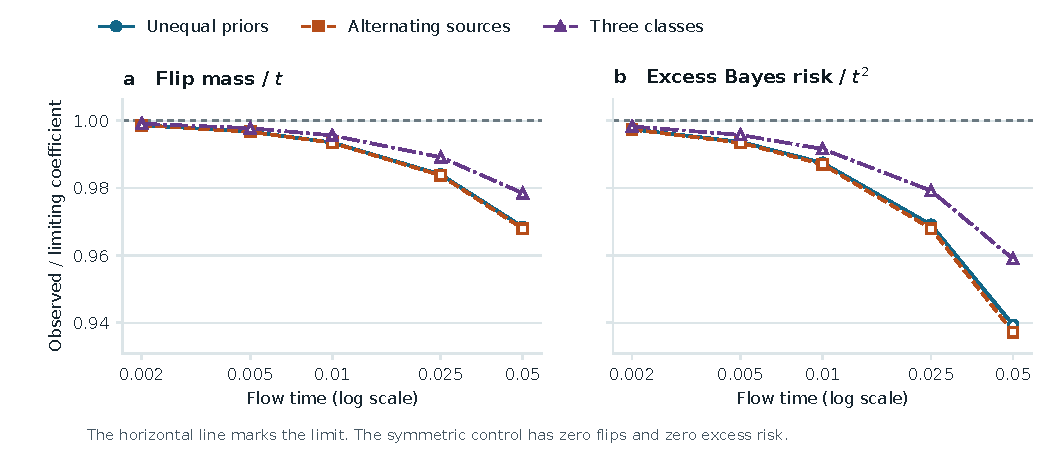
\includegraphics[width=\linewidth]{figures/oracle.pdf}
\caption{Known-law calibration. Normalizing the flip probability by $t$ and the excess Bayes risk by $t^2$ gives limits predicted from the same regular ties. The symmetric case is zero and is excluded from the ratios.}
\label{fig:oracle}
\end{figure}


\section{Discussion}
Points close to a static tie can retain their labels when the field is locally tangent or pushes them deeper into their current regions. Points farther away can change if the fitted field consistently pushes them toward another leading class. The same argument separates prediction of label changes from their usefulness. When scores approximate posterior ordering outside the core, moving points may turn correct Bayes comparisons into errors. When the ordering is biased there, a crossing can improve or degrade accuracy. Computing the effect on classification risk requires the relative density of true labels in the swept region.

The dot-product condition is local. Covariance enclosures extend it in time at an explicit cost in coverage. Concentrated posterior weights can lower the drift approximation bound. The chosen Gaussian scale and centroid geometry are part of the result's scope. Fields trained jointly with priors, adaptive anisotropic kernels, and flows that label by the ultimate equilibrium are different regimes. Machine-checked floating-point guarantees would require arithmetic enclosures in addition to the exact-arithmetic analysis.

\paragraph{Reproducibility.}
The source tree, dependency closure, data snapshots, final seeds, and decision criteria were registered before final scoring through EpistemeOS. Two locked primary jobs and two separate standard-library reanalysis jobs record the two study scopes. Per-query predictions, primary ranking scores, manifests, and verified metrics accompany the manuscript. The reanalysis uses the same recorded observations. Dataset sources and licenses are documented with the code.

\begin{thebibliography}{20}
\raggedright
\bibitem{comaniciu} D. Comaniciu and P. Meer. Mean shift: A robust approach toward feature space analysis. \emph{IEEE TPAMI}, 24(5), 2002. \href{https://doi.org/10.1109/34.1000236}{doi:10.1109/34.1000236}.
\bibitem{carreira} M. A. Carreira-Perpi\~n\'an. Gaussian mean-shift is an EM algorithm. \emph{IEEE TPAMI}, 29(5), 2007. \href{https://doi.org/10.1109/TPAMI.2007.1057}{doi:10.1109/TPAMI.2007.1057}.
\bibitem{chacon} J. E. Chac\'on. A population background for nonparametric density-based clustering. \emph{Statistical Science}, 30(4), 2015. \href{https://doi.org/10.1214/15-STS526}{doi:10.1214/15-STS526}.
\bibitem{marino} R. Marino et al. Stable attractors for neural networks classification via ordinary differential equations (SA-nODE). \href{https://arxiv.org/abs/2311.10387}{arXiv:2311.10387}, 2024.
\bibitem{kang} Q. Kang et al. Stable neural ODE with Lyapunov-stable equilibrium points for defending against adversarial attacks. \emph{NeurIPS}, 2021.
\bibitem{jem} W. Grathwohl et al. Your classifier is secretly an energy based model and you should treat it like one. \emph{ICLR}, 2020. \href{https://arxiv.org/abs/1912.03263}{arXiv:1912.03263}.
\bibitem{dupont} E. Dupont, A. Doucet, and Y. W. Teh. Augmented neural ODEs. \emph{NeurIPS}, 2019. \href{https://arxiv.org/abs/1904.01681}{arXiv:1904.01681}.
\bibitem{norcliffe} A. Norcliffe et al. On second order behaviour in augmented neural ODEs. \emph{NeurIPS}, 2020. \href{https://arxiv.org/abs/2006.07220}{arXiv:2006.07220}.
\bibitem{cox} S. M. Cox and P. C. Matthews. Exponential time differencing for stiff systems. \emph{J. Comput. Phys.}, 176(2), 2002. \href{https://doi.org/10.1006/jcph.2002.6995}{doi:10.1006/jcph.2002.6995}.
\bibitem{hochbruck} M. Hochbruck and A. Ostermann. Exponential integrators. \emph{Acta Numerica}, 19, 2010. \href{https://doi.org/10.1017/S0962492910000048}{doi:10.1017/S0962492910000048}.
\bibitem{tsuzuku} Y. Tsuzuku, I. Sato, and M. Sugiyama. Lipschitz-margin training: Scalable certification of perturbation invariance for deep neural networks. \emph{NeurIPS}, 2018. \href{https://arxiv.org/abs/1802.04034}{arXiv:1802.04034}.
\bibitem{nnvode} D. Manzanas Lopez, P. Musau, N. Hamilton, and T. T. Johnson. Reachability analysis of a general class of neural ordinary differential equations. \href{https://arxiv.org/abs/2207.06531}{arXiv:2207.06531}, 2022.
\bibitem{hall} P. Hall and K.-H. Kang. Bandwidth choice for nonparametric classification. \emph{Annals of Statistics}, 33(1), 2005. \href{https://arxiv.org/abs/math/0504511}{arXiv:math/0504511}.
\bibitem{samworth} R. J. Samworth. Optimal weighted nearest neighbour classifiers. \emph{Annals of Statistics}, 40(5), 2012. \href{https://arxiv.org/abs/1101.5783}{arXiv:1101.5783}.
\bibitem{setoudeh} F. Setoudehtazangi and G. J. McLachlan. Classification-risk-optimal label acquisition. \href{https://arxiv.org/abs/2609.06873}{arXiv:2609.06873}, 2026.
\bibitem{pendigits} E. Alpaydin and F. Alimoglu. Pen-Based Recognition of Handwritten Digits. UCI Machine Learning Repository, 1998. \href{https://doi.org/10.24432/C5MG6K}{doi:10.24432/C5MG6K}.
\bibitem{seeds} M. Charytanowicz, J. Niewczas, P. Kulczycki, P. A. Kowalski, and S. \L ukasik. Seeds. UCI Machine Learning Repository, 2010. \href{https://doi.org/10.24432/C5H30K}{doi:10.24432/C5H30K}.
\end{thebibliography}
\end{document}
